\thispagestyle{plain}
\section{Jerarqu\'ia de operaciones y signos de agrupaci\'on}
\boxabstract{Aprendizajes esperados}{
    Determina y usa la jerarquía de operaciones y los paréntesis en operaciones con números naturales, enteros y
    decimales (para multiplicación y división, sólo números positivos).
}

\subsection{Jerarqu\'ia de operaciones y signos de agrupaci\'on}
Dentro de las operaciones básicas de la aritmética existe una \textbf{jerarquía de operaciones}, es decir un
\textbf{orden}.

Recuerda cuando estabas en primaria y empezabas a leer, ¿qué aprendiste primero? Seguro fueron las vocales,
después fueron sílabas, después palabras completas hasta poder llegar a los enunciados y dentro de los enunciados
vienen los signos de puntuación, las comas, los dos puntos, el punto y seguido, el punto aparte, etc.
Y entendiste la importancia de los signos de puntuación.

En los siguientes enunciados podemos observar ejemplos:
\begin{center}
    \begin{minipage}{0.4\textwidth}
        \begin{bA}
            Perdón imposible, castigarlo.\\
            Perdón, imposible castigarlo.
        \end{bA}
    \end{minipage}
\end{center}

Como podemos ver el significado de ambas expresiones son diferentes, bueno de eso se trata, en las matemáticas
existen reglas que si no se siguen el resultado de la operación sería incorrecto.

La operación de suma, resta, multiplicación y división tienen el siguiente orden:
\begin{figure}[H]
    \centering
    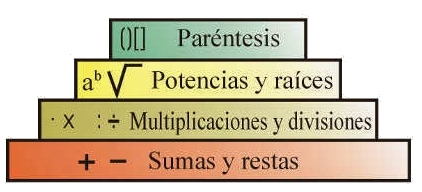
\includegraphics[width=0.5\textwidth]{./Images/jerarquia.jpg}
\end{figure}

\subsubsection{Ejemplo 1: En este ejercicio haremos uso del paréntesis}

\[( 10 + 2 ) / 3 - 2\]

Observemos en este primer ejemplo se tiene un paréntesis y tiene mayor jerarquía, por lo que primero se realiza
esta operación.

\[12 / 3 - 2\]

Seguimos con el operador que tiene la jerarquía mas alta que es la división, y vamos de izquierda a derecha y
realizamos la operación.

\[4 - 2\]

Y por último, al resultado se le restan 2. Por lo que la operación nos queda:

\[( 10 + 2 ) / 3 - 2 = 2\]



\subsubsection{Ejemplo 2: En este ejercicio no utilizaremos el paréntesis}


Ahora vamos a ver el mismo problema pero sin el paréntesis.

\[5 + 6 / 2 - 2\]

Observemos que ahora la jerarquía mas alta la tiene primero la división, ya que no existe ningún paréntesis.

\[8 + 2 - 2 = 8\]

Vamos de izquierda a derecha, hacemos primero la suma y luego la resta y tenemos el resultado, como podemos apreciar
la gran importancia de respetar el orden de las operaciones para poder encontrar el resultado correcto.


\subsubsection{Ejemplo 3: En este ejercicio explicaremos un poco más detallado}

\[4 - 6 / 2 + 5 \times 2\]

Vamos de izquierda a derecha y hacemos la división por que en este ejemplo es el operador con mas jerarquía.

\[4 - 3 + 5 \times 2\]

Luego vamos de izquierda a derecha buscando el operador que tiene la mayor jerarquía para hacer la operaci\'on.
El cual es la multiplicaciónn.

\[4 - 3 + 10\]

Seguimos con la resta por izquierda y luego por la derecha

\[1 + 10\]

Por ultimo el resultado es el número 11.

\[4 - 6 / 2 + 5 \times 2 = 11\]

\newpage


\begin{problemas}

\end{problemas}

\newpage